\subsection{Lebesgue 定理}

定理 6（Lebesgue）. --- 设 F 是一个 Banach 空间，\((\mathbf{f}_{n})\) 是 \(L_{F}^{p}\) 中函数的一个序列，使得：\(1^{\circ}\) 序列 \((\mathbf{f}_{n}(x))\) 几乎处处收敛于一个极限 \(\mathbf{f}(x) \in \mathrm{F}\) ；\(2^{\circ}\) 存在数值函数 \(g \geqslant 0\) 使 \(\int^{*} g^{p} d|\mu| < +\infty\) 且 \(|\mathbf{f}_{n}(x)| \leqslant g(x)\) 在 X 中几乎处处成立，对每个整数 n.~此时，函数 f （几乎处处有定义的）是 p 次幂可积的，且序列 \((\mathbf{f}_{n})\) p 阶平均收敛于 f。

考虑数值函数的«二重»序列 \(g_{mn} = |\mathbf{f}_m - \mathbf{f}_n|\) ，它们属于 \(\mathcal{L}^p\) （No.~5, 命题 11）；按假设，\(\lim_{m\to \infty, n\to \infty}g_{mn}(x) = 0\) 几乎处处成立，另一方面 \(|g_{mn}(x)|\leqslant 2g(x)\) 几乎处处成立；对这个二重序列应用 No.~6 定理 5 的推论 3，

\[
\limsup _ {m \to \infty ,   n \to \infty} \mathrm{N} _ {p} (\mathbf {f} _ {m} - \mathbf {f} _ {n}) \leqslant \mathrm{N} _ {p} (0) = 0  ,
\]

又由于 \(\mathrm{N}_p(\mathbf{f}_m - \mathbf{f}_n) \geqslant 0\) ，这蕴涵 \(\lim_{m \to \infty, n \to \infty} \mathrm{N}_p(\mathbf{f}_m - \mathbf{f}_n) = 0\) ；换句话说，序列 \((\mathbf{f}_n)\) 是 \(\mathcal{L}_{\mathrm{F}}^p\) 中的一个 Cauchy 序列。于是定理由 No.~4 定理 3 的推论 1 得出。

推论. --- 设 A 是一个指标集，由具有可数基的滤子 F 过滤。若 \((\mathbf{f}_{\alpha})_{\alpha \in \mathrm{A}}\) 是 \(L_{F}^{p}\) 中函数的一个族，它关于滤子 \(\mathfrak{F}\) 几乎处处逐点收敛于一个函数 \(\mathbf{f}\) ，而且若存在数值函数 \(g \geqslant 0\) 使 \(\int^{*} g^{p} d|\mu| < +\infty\) 且 \(|\mathbf{f}_{\alpha}(x)| \leqslant g(x)\) 在 \(X\) 中几乎处处成立对每个 \(\alpha \in A\) ，则函数 \(\mathbf{f}\) 是 \(p\) 次幂可积的，且 \(\mathbf{f}_{\alpha}\) 依 \(p\) 阶平均趋于 \(\mathbf{f}\) （关于滤子 \(\mathfrak{F}\) ）。

因为，设 \((\mathbf{A}_{n})\) 是 F 的一个递减可数基，并设 \(\alpha_{n}\) 是 \(A_{n}\) 中任意一个元素；序列 \((\mathbf{f}_{\alpha_{n}})\) 在 X 中几乎处处逐点收敛于 f，于是定理 6 表明 f 是 p 次幂可积的，且 \(\lim_{n\to\infty}\mathrm{N}_{p}(\mathbf{f}-\mathbf{f}_{\alpha_{n}})=0\) 。由于 F 是与所有这样的序列 \((\alpha_{n})\) 相伴的初等滤子的交滤子（GT, I, §6, No.~8, 命题 11），\(\lim_{\mathfrak{F}}\mathrm{N}_{p}(\mathbf{f}-\mathbf{f}_{\alpha})\) 存在且等于所有序列 \((\mathrm{N}_{p}(\mathbf{f}-\mathbf{f}_{\alpha_{n}}))\) 的公共极限 0。

\pandocbounded{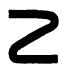
\includegraphics[keepaspectratio]{images/part001_1313f7e2.jpg}}

注记. --- 1) 若把假设 \(|\mathbf{f}_n| \leqslant g\) （其中 \(\mathrm{N}_p(g) < +\infty\) ）换成较弱的假设 \(\sup_{n} \mathrm{N}_p(\mathbf{f}_n) < +\infty\) ，定理 6 不再成立。例如，设 \(\mu\) 是 \(\mathbf{R}\) 上的 Lebesgue 测度；按下列方式定义连续函数 \(f_n\) ：\(f_n(x) = 0\) 对 \(x \leqslant 0\) 及对 \(x \geqslant \frac{2}{n}\) ，\(f_n(\frac{1}{n}) = n\) ，而 \(f_n\) 在区间 \([0, \frac{1}{n}]\) 与 \([\frac{1}{n}, \frac{2}{n}]\) 上是线性的。于是 \(\lim_{n \to \infty} f_n(x) = 0\) 对所有 \(x \in \mathbf{R}\) 成立，但 \(\mathrm{N}_1(f_n) = 1\) 对每个 \(n\) 成立（参见 §5, 习题 12）。

\pandocbounded{
\includegraphics[keepaspectratio]{images/part001_8f7b1086.jpg}}

\begin{enumerate}
\def\labelenumi{\arabic{enumi})}
\setcounter{enumi}{1}
\tightlist
\item
  若不假定滤子 \(\mathfrak{F}\) 具有可数基，定理 6 的推论不再成立（参见 §1, No.~3, 定理 3 的推论后的注记 1）。
\end{enumerate}

